
\section{Ejercicio 3 : Medici\'on de corrientes de BIAS e \textit{Input Offset Voltage}}
\subsection{Intruducci\'on}
\paragraph{Corrientes de BIAS}
Si se analiza el circuito simplificado de un amplificador operacional provisto por lo general en la hoja de datos, se puede observar que la etapa de entrada, esta compuesta por un par diferencial de transistores BJT o FET. 

Estos transistores requieren, para ser polarizados, que circule una corriente por su base, a gate. Estas corrientes son las corrientes de polarizaci\'on o BIAS,analizadas. 
 
\paragraph{Input offset voltage}
Debido al funcionamiento de la configuraci\'on en par diferencial, es de suma importancia que el balance entre ambas entradas sea correcto para que la tensi\'on a la salida de esta etapa sea 0V cuando la entrada sea 0. Esto es casi imposible de lograr sin un m\'etodo de compensaci\'on externo debido a diferencias en el comportamiento de cada uno de los transistores utilizados. 

Este desbalance genera a la salida de la etapa diferencial una tensi\'on no nula. A causa de esta, se puede ver a la salida de un amplificador operacional alimentado y con sus entradas a 0V una diferencia de potencial, llamada tensi\'on de \textit{Input Offset}

 
 
\noindent Las corrientes de  BIAS y la tensi\'on de \textit{Input Offset} son par\'ametros que dependen de la construcci\'on del amplificador operacional . Por lo general, si bien tanto las corrientes de BIAS como la tensi\'on de offset tienen valores bajos, del orden de los pA y los mV respectivamente.Sin embargo, no tenerlos en cuenta en el an\'alisis te\'orico puede llevar, en algunos casos, a resultados inesperados a la hora de analizar el comportamiento del circuito real.


\subsection{Circuito Utilizado en la medici\'on}

Se puede observar en la Figura \ref{fig:Circuito_completo} el circuito de medici\'on.

\begin{figure}[H]
   
    \centering
    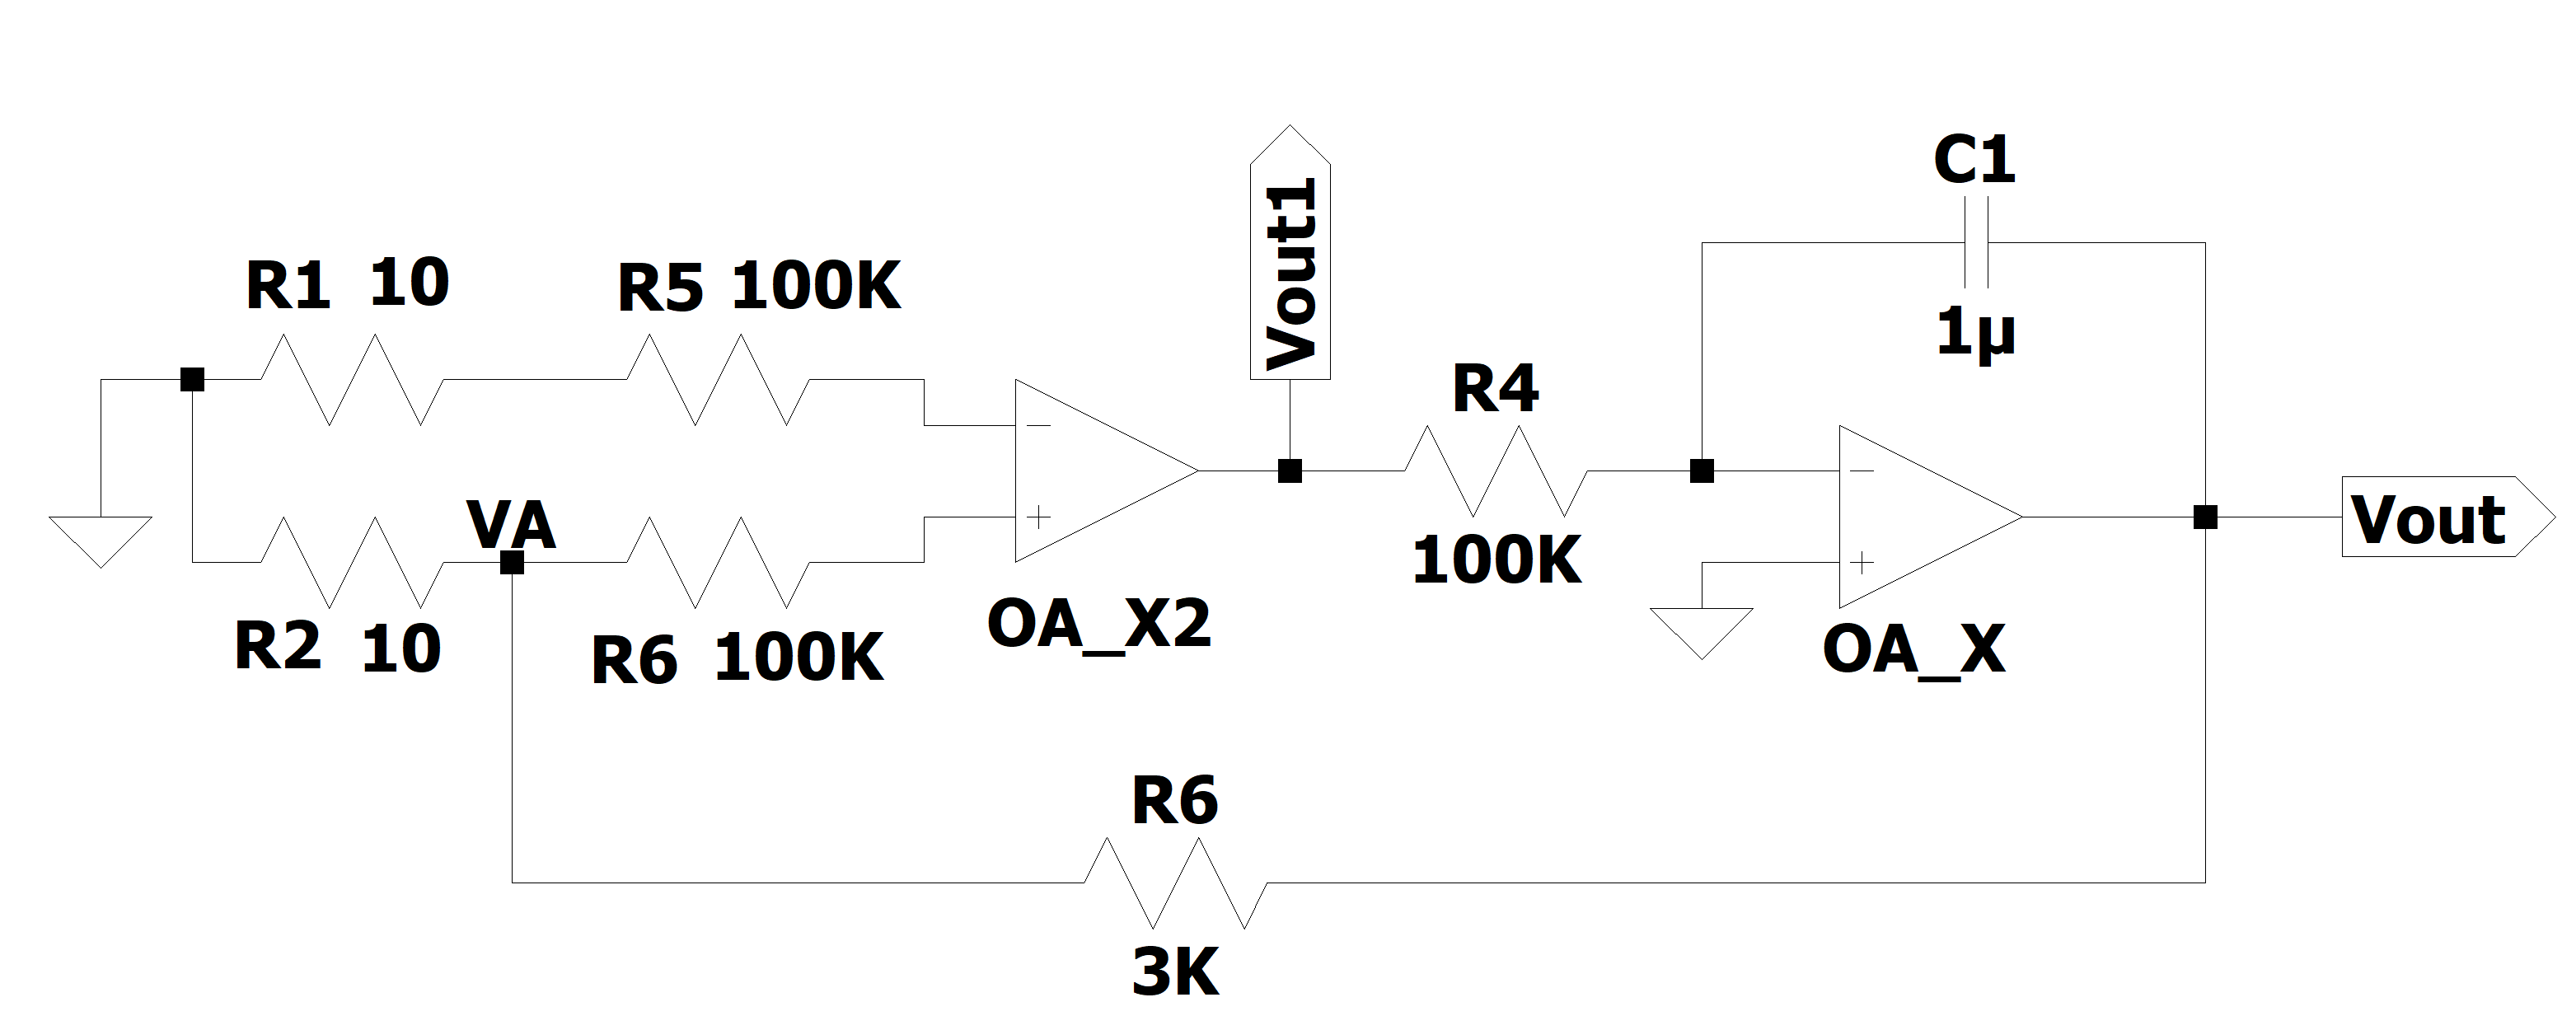
\includegraphics[width=0.5\textwidth]{../EJ3/Recursos/Circuito_completo}
    \caption{Circuito de medici\'on}
    \label{fig:Circuito_completo}
\end{figure}

Se eligen valores elevados de $R_5$ y $R_6$ para que se observe una ca\'ida de tensi\'on apreciable y se obtenga una variaci\'on observable de $V_{out}$ al cambiar la posici\'on  de SW1 y SW2. Se asigna el valor de $100K\Omega $ para las resistencias, para reducir el ruido introducido por estas al circuito, que dificultar\'ia a\'un m\'as la medici\'on.

\noindent El dispositivo que se mide es OA\_X2, por esta raz\'on $R_5$ y $R_6$ se encuentran a su entrada. 

\noindent La segunda etapa cumple la funci\'on de filtro pasabajos. Este permite que el ruido el\'ectrico que pueda haber al momento de realizar la medici\'on afecten lo menos posible a la misma. Esto es importante porque, teniendo en cuenta que las variaciones que se quieren medir estan en el orden de los mV, el nivel de ruido se haria comparable on la se\~nal a medir.
Teniendo en cuenta esto, y si se parte de la base de que el ruido que provoca mayores efectos sobre la medici\'on es el ruido de 50Hz proveniente de las l\'ineas el\'ectricas, se fija el valor de C1 en $1 \mu F$. Como se puede ver en \ref{eq:Int_end}, esto fija la frecuencia de corte del filtro que se obtiene es muy baja, de manera que para 50Hz el filtro aten\'ua aproximadamente 20dB que, en comparaci\'on a los 0,3dB de atenuaci\'on que se obtienen con el capacitor de 100nF, genera que los efectos del ruido con esa frecuencia dejan de ser tan apreciables. Lo ideal es que el valor de este capacitor sea lo m\'as grande posible analizando el circuito desde un punto de vista de las frecuencias. Sin embargo, un valor demasiado grande generar\'ia un transitorio muy lento, que requerir\'ia un tiempo largo para estabilizarse para llevar a cabo la medici\'on. Este tiempo de espera eleva la temperatura del operacional, lo que lleva a mediciones inv\'alidas.
\newline

\noindent Para realizar los c\'alculos desarrollados en esta secci\'on se deben tener en cuenta las siguientes consideraciones:
\begin{itemize}
    \item Para modelar los efectos de los fen\'omenos analizados se utiliza el modelo mostrado en la Figura \ref{fig:Modelo_BIAS}.
    
    \item Se asume para ambos operacionales en el circuito, impedancia de entrada infinita, impedancia de salida nula y ganancia a lazo abierto($A_{vol}$) finita.
    
    \item Se asume que los efectos de $I_b$ y $V_{io}$ son despreciables para la segunda etapa del circuito, por lo que solo se analizan los efectos de estas en la primera sobre todo el sistema.
    
\end{itemize}

\begin{figure}[H]
    \centering
    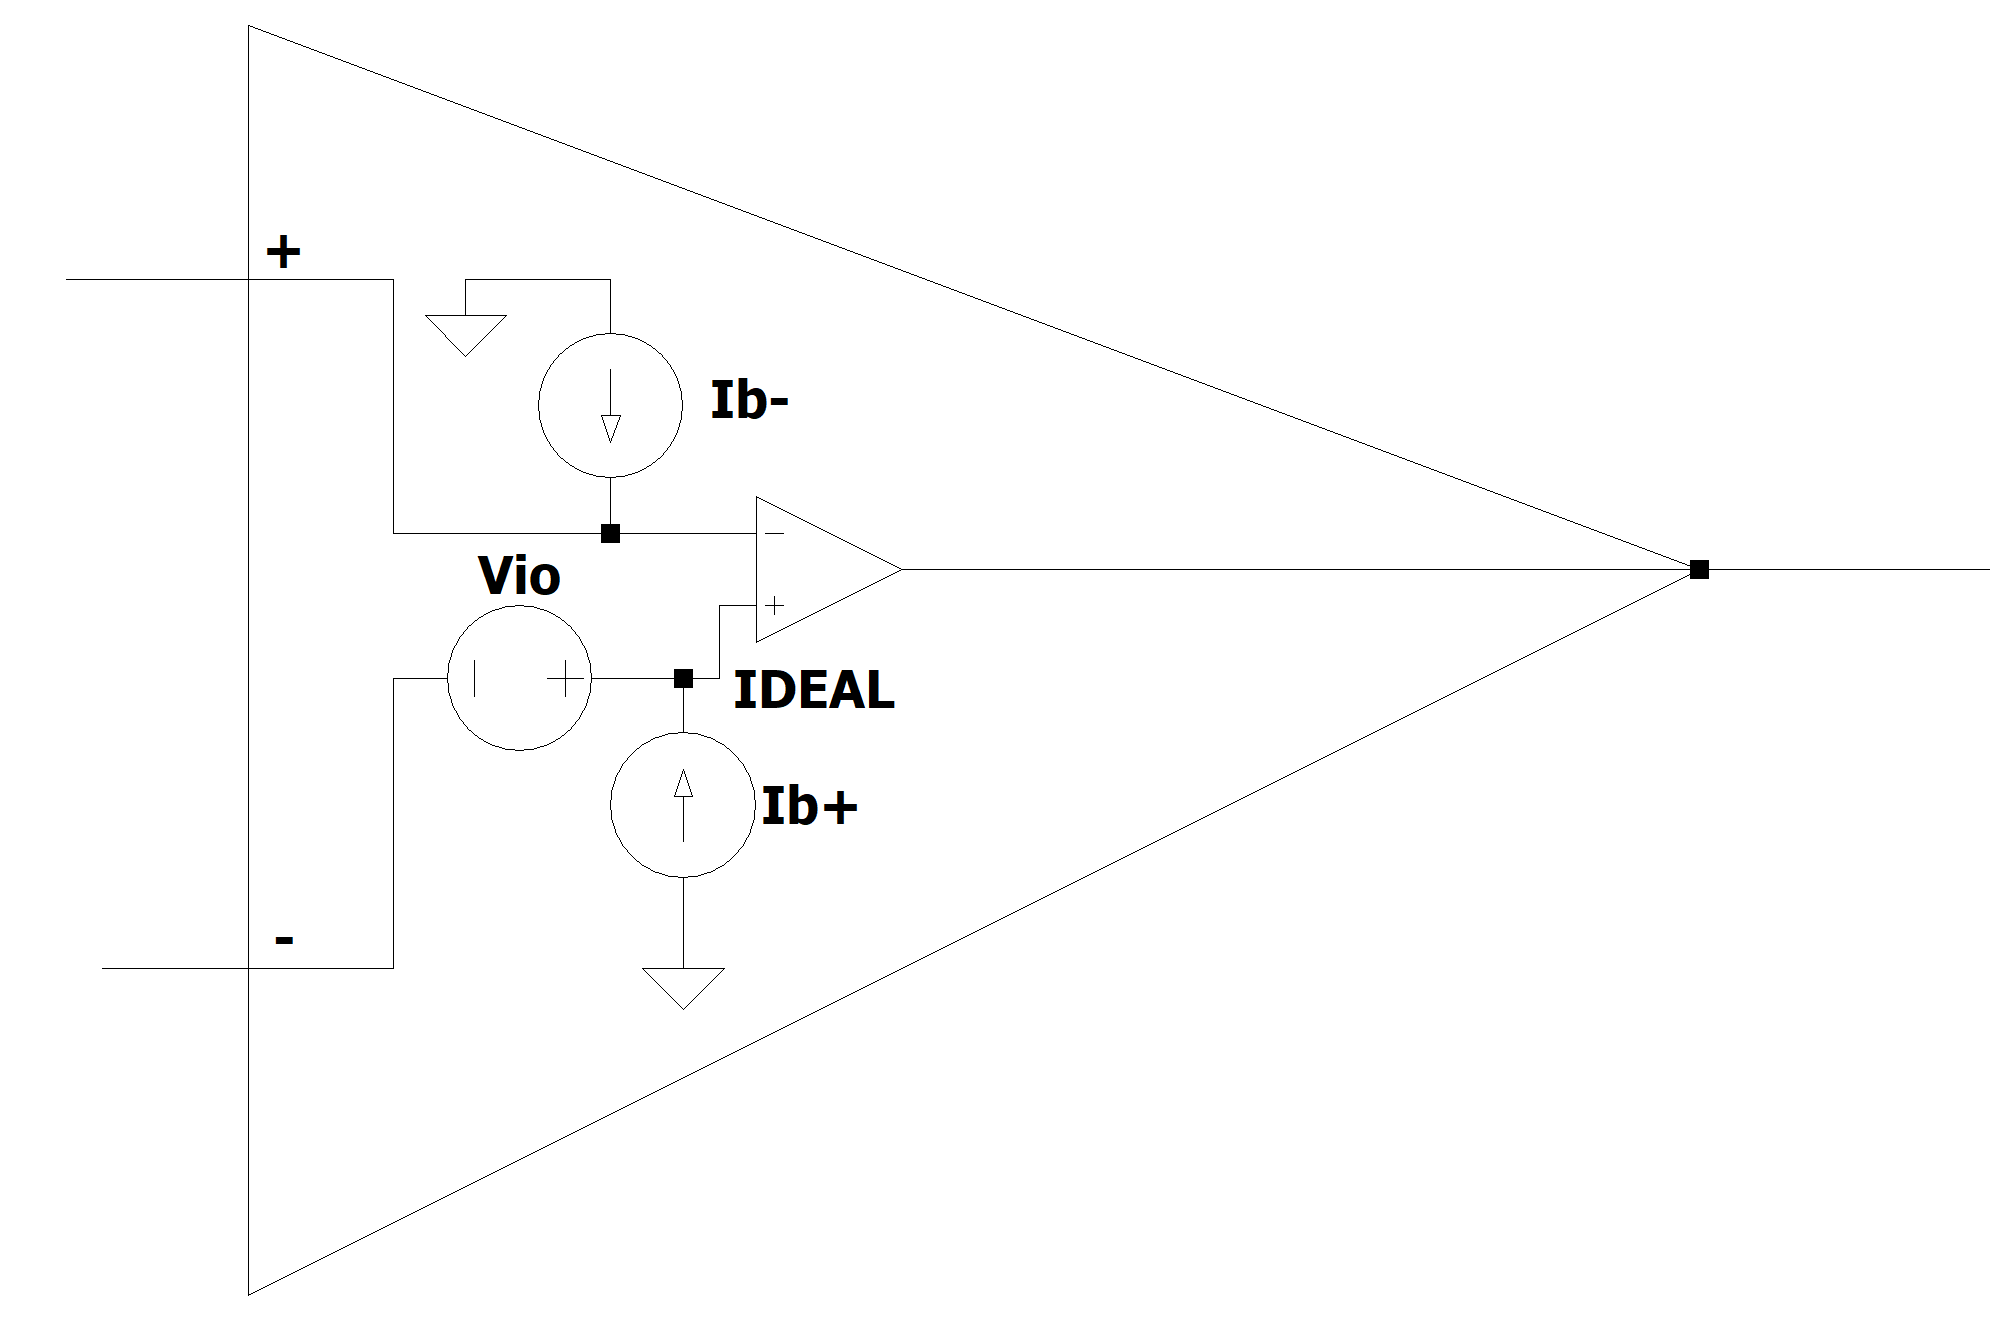
\includegraphics[width=0.5\textwidth]{../EJ3/Recursos/Modelo}
    \caption{Modelo utilizado para $I_b$ y $V_{io}$}
    \label{fig:Modelo_BIAS}
\end{figure}

\subsubsection{An\'alisis de estabilidad}

\paragraph{Segunda Etapa: Integrador}Se analiza primero la estabilidad de la segunda etapa del sistema debido a que las expresiones obtenidas al realizar el desarrollo son \'utiles para analizar la estabilidad de la primera etapa.


Se pueden observar en \ref{eq:Int_start}, las ecuaciones que describen a esta etapa.
\begin{equation}
    \left\{
    \begin{array}{lllll}
        V_{out}=A_{vol2} \cdot (V_2^+ - V_2^-)\\
        
        V_2^+ = 0 &\\
        
        V_2^- = V_{out1} - I_{R_4} \cdot R_4\\
        
        V_2^- = V_{out} - I_{C_1} \cdot \frac{1}{s\cdot C_1}\\
        
        I_{C_1} = -I_{R_4}
    \end{array}
  \right.
  \label{eq:Int_start}
\end{equation}
De operar con estas ecuaciones se obtiene \ref{eq:Int_end}, la transferencia del integrador$H(s) = \frac{ V_{out}}{V_{out1}}$ con $A_{vol2}$ finito. 
\begin{equation}
    H(s) = \frac{-A_{vol2}\cdot \frac{1}{C_1 \cdot R_4 \cdot \left(A_{vol2} + 1 \right) }}{s + \frac{1}{C_1 \cdot R_4 \cdot \left(A_{vol2} + 1 \right)}}
    \label{eq:Int_end}
\end{equation}
Se observa que el polo del sistema esta en el semiplano izquierdo del plano complejo, lo que indica que el sistema es estable.

En cambio, si se invierte la coneccion de $V_2^+$ y $V_2^-$, siguiendo un proceso an\'alogo al anterior, se obtiene \ref{eq:Int_end_unstable}
\begin{equation}
    H(s) = \frac{-A_{vol2}\cdot \frac{1}{C_1 \cdot R_4 \cdot \left(A_{vol2} - 1 \right) }}{s - \frac{1}{C_1 \cdot R_4 \cdot \left(A_{vol2} - 1 \right)}}
    \label{eq:Int_end_unstable}
\end{equation}
Donde puede verse que, en este caso, el polo del sistema se encuentra en el semiplano derecho del plano complejo, lo que genera que el sistema sea inestable.\par




\paragraph{Primera etapa: Dispositivo a probar}
Para analizar la estabilidad de esta etapa se asumen tanto SW1 como SW2 cerrados, ya que las resistencias que controlan no afectan la estabilidad. Se asume adem\'as que las corrientes de BIAS y la tensi\'on de \textit{Input Offset} son constantes, por lo que tampoco tienen ning\'un efecto sobre la estabilidad del sistema, 

Para analizar la estabilidad del sistema en este caso, se recurre a el diagrama de flujo de se\~nal. Este permite ver r\'apidamente las relaciones entre las variables del sistema y, por lo tanto, analizar su estabilidad. 
Se puede observar en la Figura \ref{fig:SFD_stable}
\begin{figure}[H]
    
    \centering
    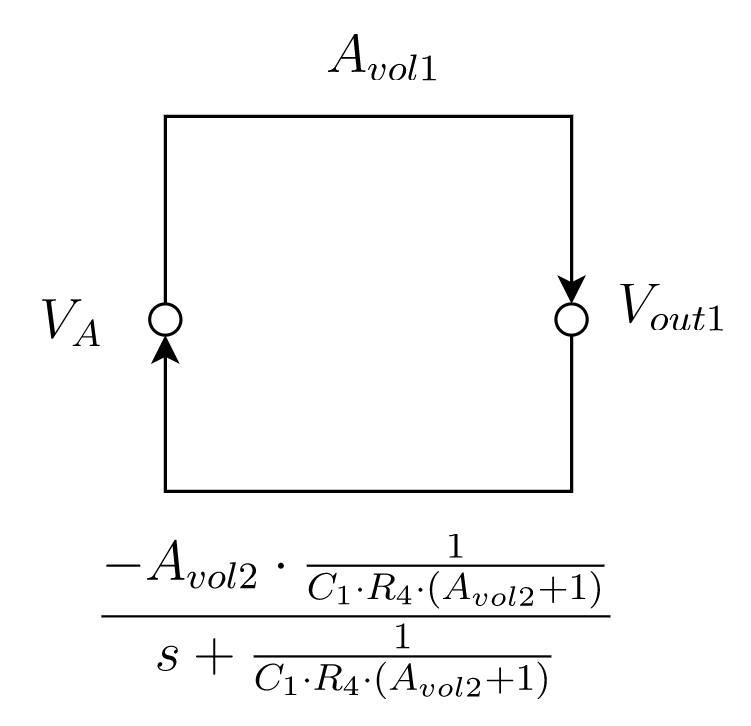
\includegraphics[width=0.5\textwidth]{../EJ3/Recursos/first_stable}
    \caption{Diagrama de flujo de se\~nal de la primera etapa en la configuraci\'on presentada}
    \label{fig:SFD_stable}
\end{figure}

Donde se ve en el diagrama una realimentaci\'on negativa, lo que hace que el sistema sea estable. Sin embargo, si se observa la Figura \ref{fig:SFD_unstable}, que representa el caso en que se invierte la conexi\'on del amplificador operacional de esta etapa, el lazo de realimentaci\'on se vuelve regenerativo, por el cambio de signo en $A_{vol1}$. Este lazo regenerativo es lo que defino que esta configuraci\'on sea inestable.
\begin{figure}[H]
   
    \centering
    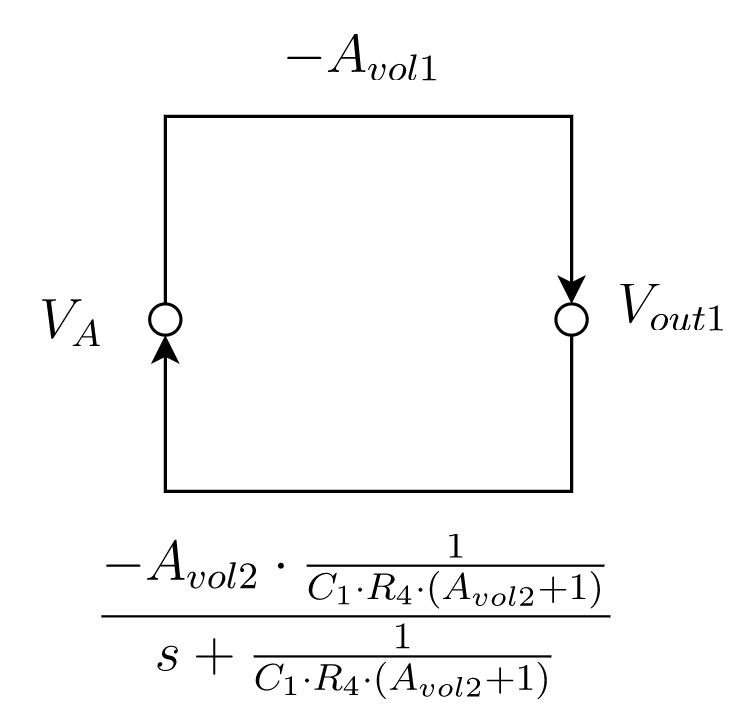
\includegraphics[width=0.5\textwidth]{../EJ3/Recursos/first_unstable}
    \caption{Diagrama de flujo de se\~nal de la primera etapa en la configuraci\'on invertida}
    \label{fig:SFD_unstable}
\end{figure}
\par
\paragraph{Invirtiendo ambas etapas}
La transferencia del sistema completo se obtiene el producto de ambas transferencias y si ninguna de las transferencias es estable, el sistema completo tampoco lo ser\'a.
\par


\subsection{An\'alisis te\'orico}
Cambiando convenientemente la combinaci\'on de SW1 y SW2 es posible calcular valores de $V_{io}$, $I_b^+$ y de $I_b^-$  como se puede observar en \ref{eq:Vio_end}, \ref{eq:Ib+_end} y \ref{eq:Ib-_end}

\paragraph{Si SW1 y SW2 est\'an cerrados}

Se asume, en este caso, que tanto las corrientes de polarizaci\'on como los efectos que estas producen en la salida son despreciables en comparaci\'on con la tensi\'on de offset. Esto debido a que al tener en la entrada del amplificador operacional una resistencia de 10$\Omega$, la diferencia de potencial generada a la entrada, se encuentra varios \'ordenes de magnitud por debajo de la tensi\'on de \textit{Input Offset} especificada por el fabricante.

Las ecuaciones que describen al sistema en este caso son las mostradas en \ref{eq:Vio_start}.
\begin{equation}
    \left\{
    \begin{array}{lllll}
        V_{out1}=A_{01} \cdot (V_1^+ - V_1^-)\\
        
        V_1^- = 0 &\\
        
        V_1^+ = V_A + V_{io}\\
        
        V_A = V_{out} \cdot \frac{R_2}{R_2 + R_3}\\
        
        V_{out} = A_{02} \cdot (V_2^+ - V_2^-)\\
        
        V_2^+ = 0
    \end{array}
  \right.
  \label{eq:Vio_start}
\end{equation}

De operar con estas ecuaciones se obtiene \ref{eq:Vio_end} que permite obtener un valor de la tensi\'on de \textit{Input Offset} a partir de medir la tensi\'on a la salida del sistema.

\begin{equation}
    V_{io} = -V_{out} \cdot \left(\frac{1}{A_{01} \cdot A_{02}} + \frac{R_2}{R_2+R_3}\right)
    \label{eq:Vio_end}
\end{equation}
Y si se asume que $A_{vol1} \cdot A_{vol2} \gg 1$, se desprecia el primer t\'ermino de la suma y el sistema se independiza de los $A_{vol}$ de los operacionales. 
\par

\paragraph{Si SW1 est\'a cerrado y SW2 abierto}

Se asume nuevamente que las corrientes de BIAS son lo suficientemente peque\~nas para despreciar sus efectos antes de la resistencia $R_6$. Sin embargo, en este caso, la corriente $I_b^+$ en conjunto con $R_6$ generan una diferencia de potencial que genera a la salida del sistema una variaci\'on observable.
Las ecuaciones que describen al sistema en este caso son las mostradas en \ref{eq:Ib+_start}.
\begin{equation}
    \left\{
    \begin{array}{lllll}
        V_{out1}=A_{01} \cdot (V_1^+ - V_1^-)\\
        
        V_1^- = 0 &\\
        
        V_1^+ = V_A + V_{io} + I_b^+ \cdot R_6 \\
        
        V_A = V_{out} \cdot \frac{R_2}{R_2 + R_3}\\
        
        V_{out} = A_{02} \cdot (V_2^+ - V_2^-)\\
        
        V_2^+ = 0
    \end{array}
  \right.
  \label{eq:Ib+_start}
\end{equation}
De operar con estas ecuaciones se obtiene \ref{eq:Ib+_end} que permite obtener un valor de $I_b^+$ a partir de medir la tensi\'on a la salida del sistema.
\begin{equation}
    I_b^+ = \frac{ -V_{out} \cdot \left(\frac{1}{A_{01} \cdot A_{02}} + \frac{R_2}{R_2+R_3}\right) - V_{io}}{R_6}
    \label{eq:Ib+_end}
\end{equation}
Y si se asume que $A_{vol1} \cdot A_{vol2} \gg 1$, se desprecia el primer t\'ermino de la suma y el sistema se independiza de los $A_{vol}$ de los operacionales.
\par

\paragraph{Si SW1 est\'a abierto y SW2 cerrado}

De manera an\'aloga al caso anterior se obtiene \ref{eq:Ib-_end}
\begin{equation}
    I_b^- = \frac{ V_{out} \cdot \left(\frac{1}{A_{01} \cdot A_{02}} + \frac{R_2}{R_2+R_3}\right) + V_{io}}{R_1 + R_5}
    \label{eq:Ib-_end}
\end{equation}

\par

\subsection{Mediciones y an\'alisis de resultados}
Se pueden observar los resultados de las mediciones realizadas tanto para el TL081 como para el LF356 en las Tablas \ref{tab:TL081_res} y \ref{tab:LF356_res} respectivamente.
\begin{table}[H]
    \centering
    \resizebox{0.5\textwidth}{!}{%
    \begin{tabular}{llllll}
        \hline
        \multicolumn{6}{|c|}{TL081} \\ 
        \hline \\ 
        SW1 & SW2 & $V_{out}(mV)$ & $V_{io}(\mu V)$ & $I_b^+(pA)$ & $I_b^-(pA)$ \\ 
        \hline  \\ 
        cerrado & cerrado & 219 & -728 & - & - \\
        cerrado & abierto & 223 & - & -130 & - \\
        abierto & cerrado & 217 & - & - & -80 \\
        \hline
    \end{tabular}
    }
    \caption{Resultados de las mediciones realizadas para el TL081}
    \label{tab:TL081_res}
\end{table}


\begin{table}[H]
\centering
\resizebox{0.5\textwidth}{!}{%
\begin{tabular}{cccccc}
\hline
\multicolumn{6}{|c|}{LF356} \\ \hline
SW1 & SW2 & $V_{out}(mV)$ & $V_{io}(\mu V)$ & $I_b^+(pA)$ &$ I_b^-(pA)$ \\ \hline
cerrado & cerrado  & -250 & 832 & - &  \\
cerrado  & abierto & -245 & - & 199 & - \\
abierto & cerrado  & -256 & - & - & 193 \\ \hline
\end{tabular}%
}
\caption{\label{tab:LF356_res} Resultados de las mediciones realizadas para el LF356}
\end{table}
Se observa que el valor t\'ipico de tensi\'on de offset provisto por el fabricante\footnote{Informaci\'on tomada de las respectivas hojas de datos, disponibles en el sitio de Texas Instruments, http://www.ti.com} para ambos amplificadores operacionales es de 3mV. Los valores obtenidos se encuentran por debajo de este valor, estando ambos por debajo de 1mV.

\noindent Para el an\'alisis de los valores de las corrientes, se muestra  en \ref{eq:Ib_def} la forma en la que el fabricante presenta estos par\'ametros en la hoja de datos. 
\begin{equation}
    \centering
    \left.
    \begin{array}{ll}
        I_{OS} /I_{io} = \left| I_b^+ - I_b^- \right|, \textit{Input offset current} \\
        I_B = \frac{I_b^+ + I_b^- }{2}, \textit{Input BIAS current}
    \end{array}
    \right.
  \label{eq:Ib_def}
\end{equation}
En el caso del TL081 los valores obtenidos al realizar estos c\'alculos son de $I_{io} =50pA $ y $I_B = 105pA$ ambos dentro del rango se\~nalado en la hoja de datos, de 100pA y 200pA como m\'aximo, respectivamente. A pesar de esto se observa una desviaci\'on considerable del valor t\'ipico, de 5pA y 30pA respectivamente.
\\\\
En cambio para el LF356 se obtienen valores de $I_{io} =6pA $ y $I_B = 196pA$. En este caso, si bien ambos valores se encuentran en el rango aceptado por el fabricante, el valor de $I_B$ es muy cercano al valor m\'aximo aceptable.
\\\\
Las diferencias con los valores de la hoja de datos se atribuye en parte  a errores procedurales al realizar la medici\'on. Esto se debe a que el fabricante especifica que para realizarla, se debe conectar la alimentaci\'on del amplificador operacional a pulsos, dada la fuerte incidencia que las variaciones temperaturas de juntura, en particular luego de $25^\circ C$, tienen sobre estas corrientes.

Adem\'as, otra posible fuente de error, se encuentra en las peque\~nas variaciones de las tensiones de salida en comparaci\'on con el ruido el\'ectrico ambiente que, a pesar de haber aumentado el valor del capacitor, a\'un ten\'ia efectos notables en la salida.

\subsubsection{Compensaci\'on externa para un amplificador operacional en configuraci\'on inversora}
Se presenta a continuaci\'on una posible opci\'on para un circuito que permite, en un amplificador operacional en configuraci\'on inversora como el de la Figura \ref{fig:Inversor}, reducir los efectos que las corrientes de BIAS tienen en la salida del circuito. Se decide en este caso considerar \'unicamente el caso de $A_{vol}$ infinito para simplificar el desarrollo.
\begin{figure}[H]
    
    \centering
    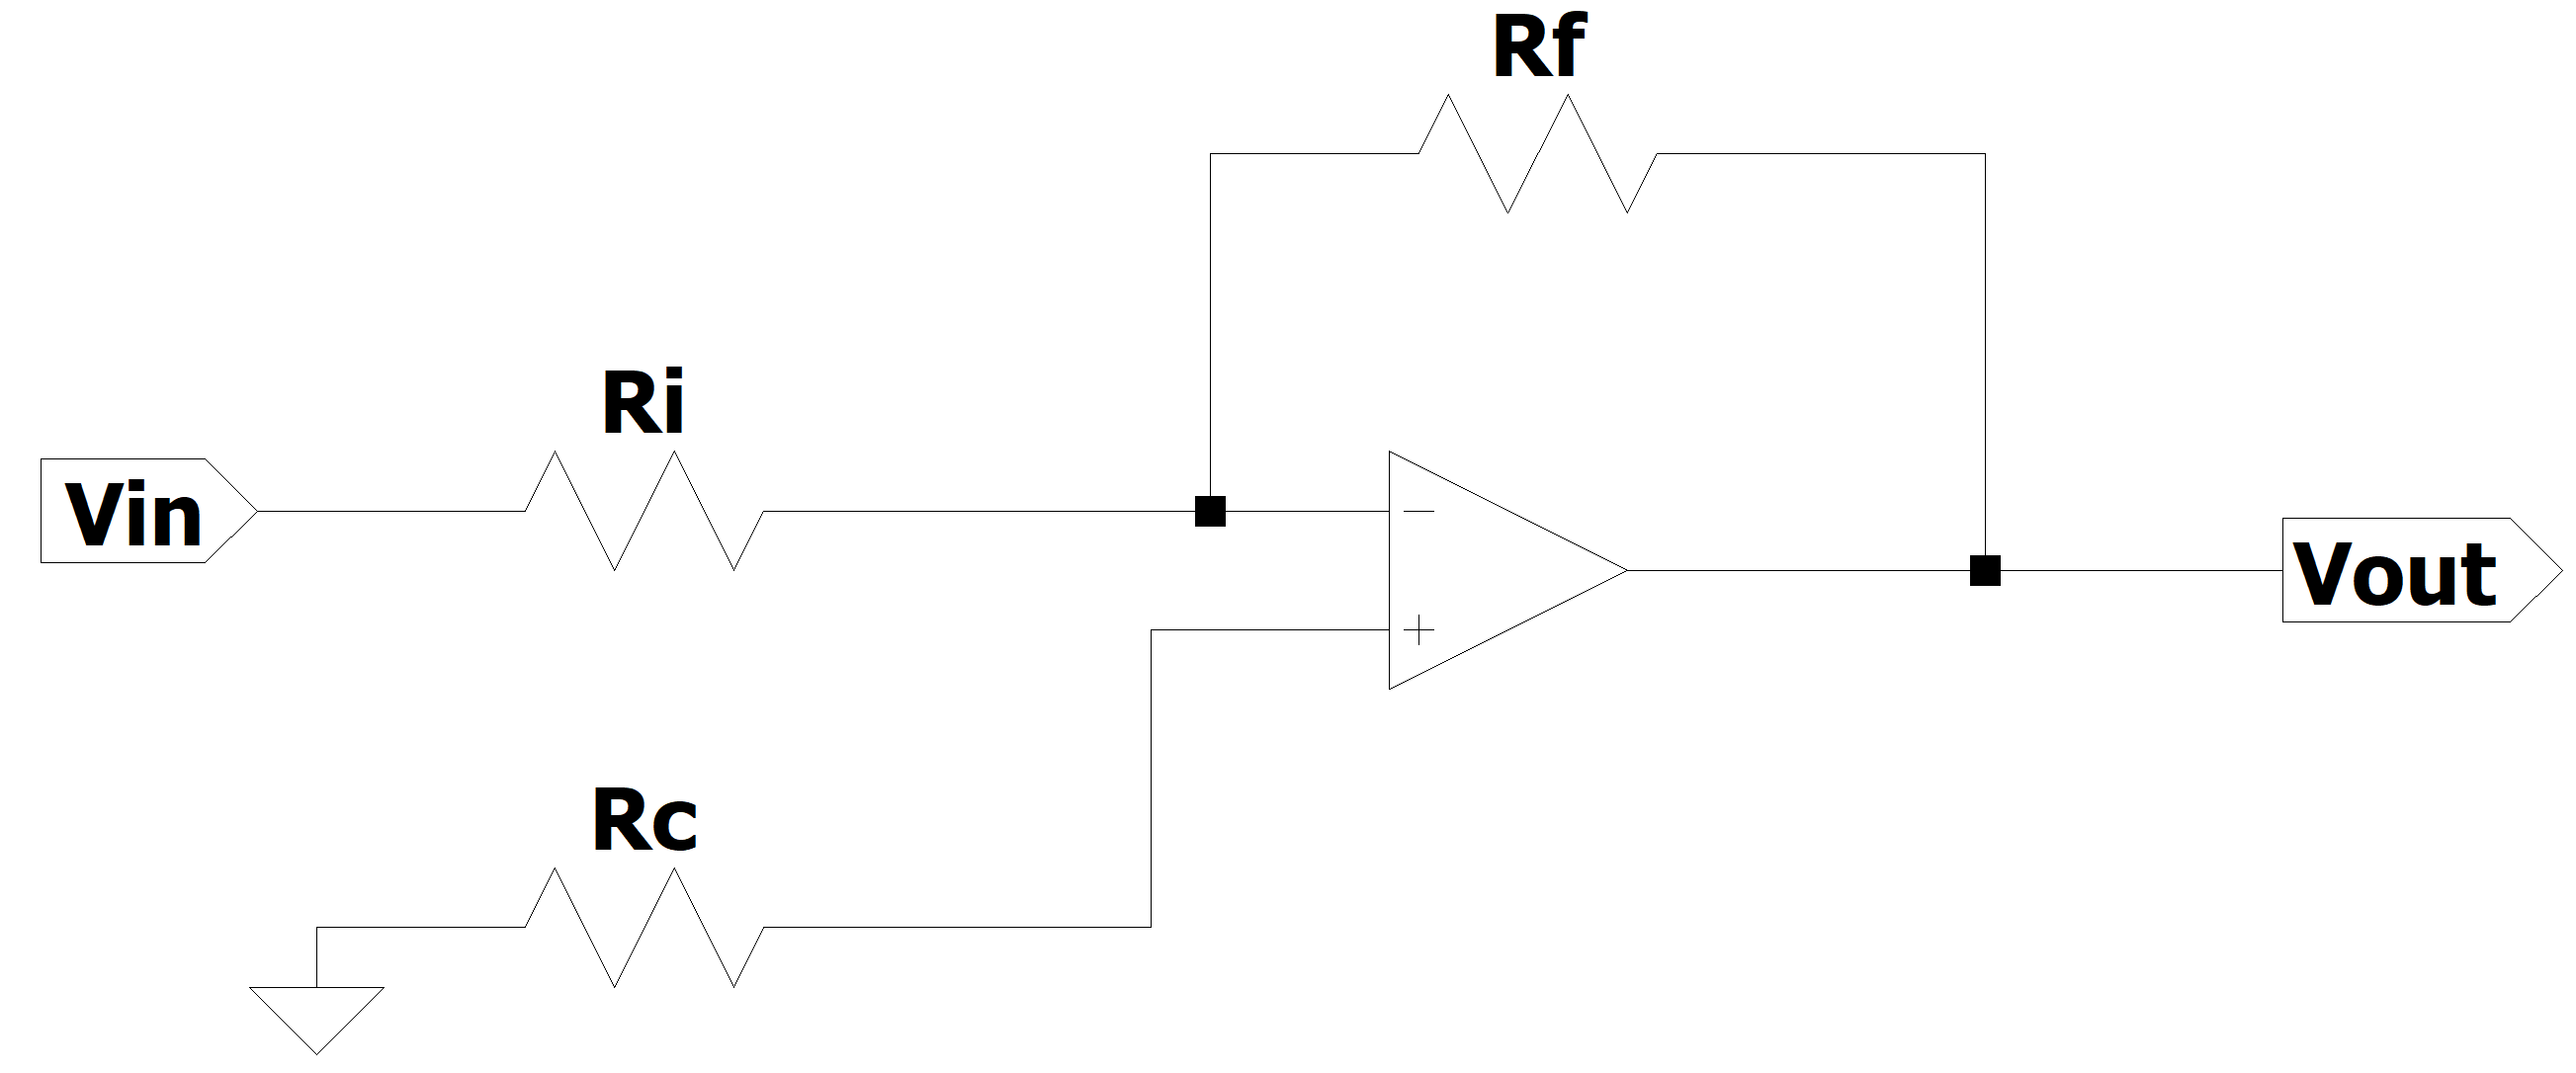
\includegraphics[width=0.5\textwidth]{../EJ3/Recursos/Inversor}
    \caption{\label{fig:Inversor}Amplificador inversor}
\end{figure}
Si se conecta la entrada a GND y se aplica superposici\'on para obtener solamente los efectos producidos por las corrientes de BIAS en la salida, teniendo en cuenta el modelo presentado en la Figura \ref{fig:Modelo_BIAS}.

Se obtiene entonces \ref{eq:voi_ibs}, que permite realacionar los valores de resistencia y los valores de $I_b^+$ \'e $I_b^-$, con la tensi\'on de salida en las condiciones descriptas, que se nombra $V_{out_{I_b's}}$.

\begin{equation}
    V_{out_{I_b's}} = \left|R_c \cdot I_b^+ \cdot \left( 1+\frac{R_f}{R_i}\right) - R_f \cdot I_b^-\right|
    \label{eq:voi_ibs}
\end{equation}

Se asume que las corrientes de BIAS tienen el mismo valor. Si bien, como se puede observar en las mediciones no es correcto, permite realizar una primera aproximaci\'on.

Bajo esta condici\'on y si se cumple que $R_c = R_i//R_f$, la tensi\'on a la salida del operacional sin nada a la entrada es 0V y no se observan las diferencias por las corrientes de offset en el funcionamiento del circuito.
Por \'ultimo, para corregir la tensi'on de offset, que al resolver por superposici\'on no se tuvo en cuenta, se propone el circuito de la Figura \ref{fig:Off_comp}.
\begin{figure}[H]
    
    \centering
    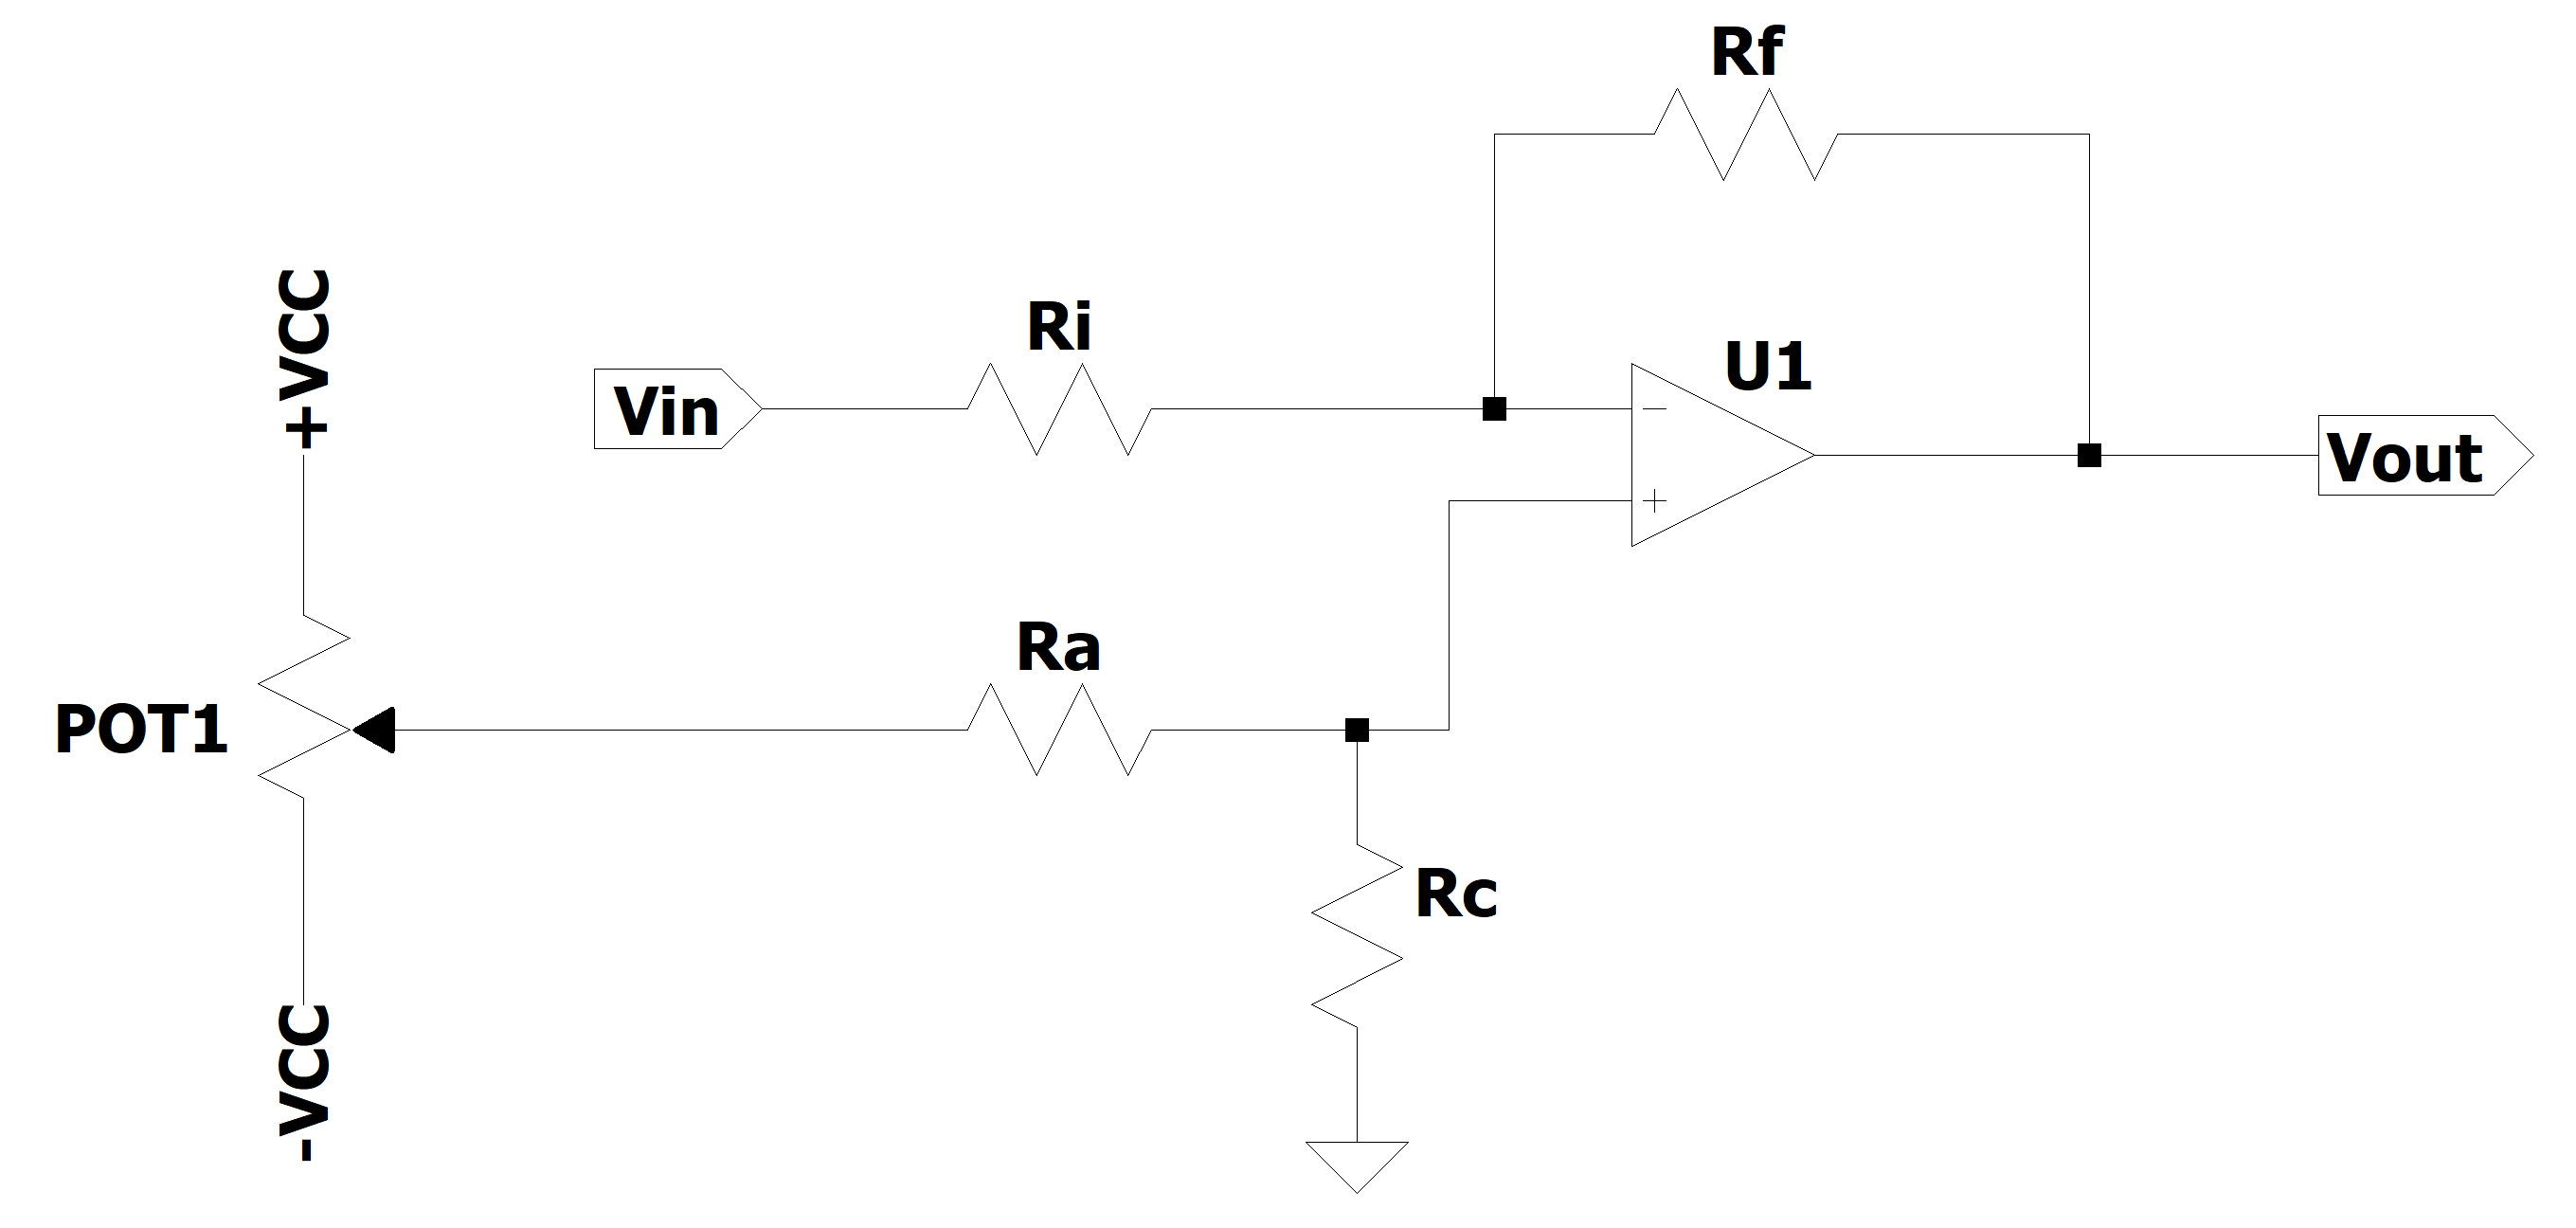
\includegraphics[width=0.5\textwidth]{../EJ3/Recursos/Off_comp}
    \caption{\label{fig:Off_comp}Amplificador inversor con circuito de compensaci\'on de tensi\'on de offset }
\end{figure}

Eligiendo valores convenientes para $R_a$, en particular que se cumpla que $R_a \gg R_c$, y para el potenci\'ometro, es posible compensar la tensi\'on $V_io$ aplicando una tensi\'on igual pero de signo opuesto.
Es importante que se cumpla $R_a \gg R_c$ debido a que $V_io$ esta en el orden de los mV, y dada esta condici\'on se puede ver que la tensi\'on de compensaci\'on se calcula como $V_{comp} \approx V_{pot}\cdot \frac{R_a}{R_c}$.
  